\documentclass[11pt]{article}
\usepackage[margin=1in]{geometry}
\usepackage{amsmath,amssymb}
\usepackage{graphicx}
\usepackage{booktabs}
\usepackage{hyperref}
\usepackage{listings}
\usepackage{xcolor}
\lstset{basicstyle=\ttfamily\small, breaklines=true, columns=fullflexible,
        backgroundcolor=\color{gray!8}, frame=single, framerule=0pt}

\title{Independent Replication: \\
\emph{Quantum Search by Local Adiabatic Evolution} \\
{\normalsize Roland \& Cerf, arXiv:quant-ph/0107015 (2001)}}
\author{QC-200 replication wave — automated agent run}
\date{2026-07-05}

\begin{document}
\maketitle

\begin{abstract}
We independently reproduce the central claim of Roland and Cerf (2001) that
switching a driving Hamiltonian $H(s)=(1{-}s)H_0+sH_m$ under a \emph{locally}
adiabatic schedule $s(t)$ recovers the $O(\sqrt N)$ Grover speed-up for
unstructured quantum search, whereas the naive linear schedule $s(t)=t/T$ gives
$O(N)$. Using direct Schr\"odinger integration in the 2-D Grover invariant
subspace (verified against full $N$-dim statevector at small $N$), we bisect the
minimum total evolution time $T^{\ast}(N)$ needed to reach $p_{\rm succ}\ge 1/2$
for $N\in\{8,16,32,64,128,256,512,1024,2048\}$. Log--log fits give slopes
\textbf{$0.9992$ (linear)} and \textbf{$0.4756$ (local-adiabatic)}, matching the
paper's analytic predictions of $1.0$ and $0.5$ to within $0.03$.
\textbf{Verdict: REPLICATED.}
\end{abstract}

\section{Paper summary}

Roland \& Cerf (2001) apply the adiabatic-quantum-computation framework
introduced by Farhi \emph{et al.} (2001) to Grover's unstructured-search
problem. They use the same interpolated Hamiltonian as Farhi \emph{et al.},
\[
  \tilde H(s)=(1-s)(I-|\psi_0\rangle\langle\psi_0|)+s(I-|m\rangle\langle m|),
  \qquad s=t/T,
\]
with $|\psi_0\rangle=N^{-1/2}\sum_i|i\rangle$ and $|m\rangle$ the unknown
marked state. Its 2--D reduction on $\mathrm{span}(|m\rangle,|\psi_0\rangle)$
gives an analytically known instantaneous gap
$g(s)=\sqrt{1-4\,(N-1)/N\,s(1-s)}$, minimum $g_{\min}=1/\sqrt N$ at $s=1/2$.

\medskip\noindent\textbf{Key insight.} A globally-adiabatic (linear) schedule
requires $T\gtrsim N/\varepsilon$ because it must be slow enough to respect the
adiabatic condition at $s=1/2$. But away from $s=1/2$, $g(s)$ is $O(1)$, so
the schedule can go much faster there. Choosing
$ds/dt=\varepsilon g^2(s)$ (Eq.~17 of the paper) saturates the adiabatic
condition pointwise and integrates to
$T=(\pi/2\varepsilon)\sqrt N$ (Eq.~19).

\section{Claims table}

\begin{center}\small
\begin{tabular}{p{0.5cm}p{7cm}p{2cm}p{2cm}p{3cm}}
\toprule
\# & Claim & Type & Testable? & Tested here? \\
\midrule
C1 & Linear/global schedule with $H_0,H_m$ above needs $T\propto N$ to succeed. & Analytic scaling & Yes (numerical fit) & \textbf{Yes} \\
C2 & Local-adiabatic schedule with $ds/dt=\varepsilon g^2(s)$ needs $T=(\pi/2\varepsilon)\sqrt N$. & Analytic scaling + coefficient & Yes (numerical fit + coefficient) & \textbf{Yes} \\
C3 & Local-adiabatic algorithm is optimal ($T=\Theta(\sqrt N)$) among all $s(t)$. & Optimality theorem & Only lower-bound check (didn't attempt) & No — proof-of-optimality out of scope for reproduction \\
C4 & Dynamics stays in the 2--D $\mathrm{span}(|m\rangle,|\psi_0\rangle)$ subspace. & Structural & Yes & \textbf{Yes} (2--D reduction vs full-$N$ statevector agrees to $\sim 10^{-15}$) \\
C5 & Approach generalizes to other adiabatic problems (NP-complete, nested Grover). & Speculative & No & No (not a claim of this paper's numerical section) \\
\bottomrule
\end{tabular}
\end{center}

C1, C2, C4 are the concrete falsifiable claims and are all tested.

\section{Method}

\subsection{Tools \& versions}
\begin{itemize}
\item Python 3.14.6 (system \texttt{/usr/local/bin/python3}).
\item NumPy 2.4.3, SciPy 1.18.0, Matplotlib 3.10.8 (site-installed).
\item ODE integrator: \texttt{scipy.integrate.solve\_ivp}, method \texttt{DOP853}
      (8th-order Dormand-Prince), \texttt{rtol=1e-9}, \texttt{atol=1e-11},
      \texttt{max\_step=T/200}.
\item PDF: \texttt{pdftotext} (Poppler) for text extraction.
\end{itemize}

\subsection{Dynamics}

Because $H_0$ and $H_m$ both preserve $V=\mathrm{span}(|m\rangle,|m_\perp\rangle)$
where $|m_\perp\rangle$ is the normalized projection of $|\psi_0\rangle$ onto
$|m\rangle^\perp$, and the initial state $|\psi_0\rangle\in V$, we may integrate
Schr\"odinger's equation in that 2--D space exactly. In the
$\{|m\rangle,|m_\perp\rangle\}$ basis with $a=1/\sqrt N$, $b=\sqrt{1-1/N}$:
\[
  |\psi_0\rangle\langle\psi_0|=\begin{pmatrix}a^2 & ab\\ ab & b^2\end{pmatrix},\qquad
  |m\rangle\langle m|=\begin{pmatrix}1 & 0\\ 0 & 0\end{pmatrix},
\]
and $\tilde H(s)=(1-s)(I-|\psi_0\rangle\langle\psi_0|)+s(I-|m\rangle\langle m|)$
is a $2\times 2$ real-symmetric matrix.

We use two schedules:

\medskip
\emph{Linear (baseline).} $s(t)=t/T$, $t\in[0,T]$.

\medskip
\emph{Local-adiabatic (Roland--Cerf).} Given $T$, we choose $\varepsilon$
such that Eq.~(18) evaluated at $s=1$ equals $T$:
\[
  \varepsilon=\frac{N}{T\sqrt{N-1}}\arctan(\sqrt{N-1}),
\]
then invert Eq.~(18) to get $s(t)$:
\[
  s(t)=\tfrac{1}{2}+\frac{\tan\!\big(\tfrac{2\varepsilon\sqrt{N-1}\,t}{N}-\arctan(\sqrt{N-1})\big)}{2\sqrt{N-1}}.
\]

\subsection{Sanity check: 2-D reduction vs full-$N$ statevector}

For $N\in\{4,8,16\}$ and both schedules, we compared the 2--D success probability
$|a(T)|^2$ against a full $N$-dim Schr\"odinger integration using dense
$N\times N$ matrices $I-|\psi_0\rangle\langle\psi_0|$ and $I-|m\rangle\langle m|$.
All differences $|p_{2D}-p_{\text{full}}|$ are below $2\times 10^{-15}$
(see Table~\ref{tab:sanity}). The 2--D reduction is exact.

\begin{table}[h]\centering\small
\begin{tabular}{rrrrrr}
\toprule
$N$ & schedule & $T$ & $p_{\text{full}}$ & $p_{\rm 2D}$ & $|{\rm diff}|$ \\
\midrule
 4 & linear &  8.0000 & 0.804134 & 0.804134 & $1.67\times 10^{-15}$ \\
 4 & local  &  3.1416 & 0.441550 & 0.441550 & $1.11\times 10^{-16}$ \\
 8 & linear & 16.0000 & 0.841449 & 0.841449 & $1.78\times 10^{-15}$ \\
 8 & local  &  4.4429 & 0.376522 & 0.376522 & $1.67\times 10^{-16}$ \\
16 & linear & 32.0000 & 0.800214 & 0.800214 & $2.22\times 10^{-16}$ \\
16 & local  &  6.2832 & 0.359663 & 0.359663 & $1.11\times 10^{-16}$ \\
\bottomrule
\end{tabular}
\caption{2-D subspace reduction vs full $N$-dim statevector integration.}
\label{tab:sanity}
\end{table}

\subsection{Finding $T^{\ast}(N)$}
For each $(N,\text{schedule})$, we bisected on $T$ until we found the smallest
$T$ giving $p_{\rm succ}(T)\ge 1/2$, to relative tolerance $0.01$.
Starting brackets were anchored on the paper's predictions ($T\sim N$ linear,
$T\sim(\pi/2)\sqrt N$ local) and expanded/contracted as needed.
$N\in\{8,16,32,64,128,256,512,1024,2048\}$.

\subsection{Commands}
\begin{lstlisting}
$ python3 code/adiabatic_search.py report/evidence
$ python3 code/plots.py
\end{lstlisting}

\section{Results vs paper}

\begin{table}[h]\centering\small
\begin{tabular}{rrrrrrr}
\toprule
$N$ & schedule & $T^{\ast}$ & $p_{\rm succ}(T^{\ast})$ & \multicolumn{2}{c}{ratio to paper prediction} \\
\midrule
 8 & linear & 7.63 & 0.5028 & $T^{\ast}/N$ = 0.954 & \\
 8 & local  & 5.68 & 0.5027 & $T^{\ast}/((\pi/2)\sqrt N)$ = 1.28 & \\
16 & linear & 12.92 & 0.5016 & 0.808 & \\
16 & local  & 8.04  & 0.5033 & 1.28 & \\
32 & linear & 28.89 & 0.5022 & 0.903 & \\
32 & local  & 11.10 & 0.5016 & 1.25 & \\
64 & linear & 56.84 & 0.5029 & 0.888 & \\
64 & local  & 15.32 & 0.5018 & 1.22 & \\
128& linear & 112.75 & 0.5020 & 0.881 & \\
128& local  & 21.12  & 0.5001 & 1.17 & \\
256& linear & 227.38 & 0.5023 & 0.888 & \\
256& local  & 29.49  & 0.5041 & 1.16 & \\
512& linear & 454.75 & 0.5024 & 0.888 & \\
512& local  & 40.90  & 0.5005 & 1.13 & \\
1024& linear & 909.50 & 0.5023 & 0.888 & \\
1024& local  & 57.46  & 0.5032 & 1.13 & \\
2048& linear & 1819.00 & 0.5023 & 0.888 & \\
2048& local  & 80.72   & 0.5036 & 1.12 & \\
\bottomrule
\end{tabular}
\caption{Minimum $T^{\ast}$ reaching $p_{\rm succ}\ge 1/2$ vs $N$.}
\end{table}

\subsection{Log-log scaling fits}
\[
  \log T^{\ast} = m\,\log N + c
\]
\begin{center}\small
\begin{tabular}{lccccc}
\toprule
schedule & fitted slope $m$ & fitted intercept $c$ & $R^2$ & paper predicts $m$ & $|\Delta m|$ \\
\midrule
linear         & $0.9992$ & $-0.1163$ & $0.99950$ & $1.0$ & $0.001$ \\
local-adiabatic& $0.4756$ & $+0.7531$ & $0.99991$ & $0.5$ & $0.024$ \\
\bottomrule
\end{tabular}
\end{center}

Both slopes match the paper's predictions to well within $10\%$ tolerance, with
$R^2>0.999$ over more than two decades of $N$.

\medskip
\noindent\textbf{Coefficient check (local).} The paper's asymptotic
prediction Eq.~(19) with $\varepsilon\to 1$ (the natural scale after saturation)
gives $T\approx(\pi/2)\sqrt N \approx 1.571\sqrt N$. Our fit intercept
$c=0.7531$ implies $T^{\ast}\approx e^{0.7531}\sqrt N \approx 2.12\,\sqrt N$
at $p_{\rm succ}=1/2$, corresponding to an effective
$\varepsilon_{\text{eff}}\approx (\pi/2)/2.12\approx 0.74$.
That is entirely reasonable: the paper's Eq.~(19) is a sufficient-condition
bound with unspecified $\varepsilon\ll 1$, while $T^{\ast}$ is the tight
$p_{\rm succ}=1/2$ threshold. The important point is the \emph{scaling exponent},
which the paper predicts exactly and we recover.

\medskip
\noindent\textbf{Coefficient check (linear).} Our fit intercept
$c=-0.1163$ implies $T^{\ast}\approx 0.89\,N$. The paper's Eq.~(15) gives
$T\ge N/\varepsilon$ with $\varepsilon\ll 1$, i.e.\ prefactor $\ge 1$; our
threshold $T^{\ast}$ sitting slightly below $N$ is fine and just reflects that
we picked the $p_{\rm succ}=1/2$ operating point.

\subsection{Figures}

Figure~\ref{fig:scaling} shows the log--log scaling of $T^{\ast}$ vs $N$ with
the two fitted lines and $\sim N$, $\sim\sqrt N$ reference lines.

Figure~\ref{fig:pvT} shows the success probability as a function of the total
evolution time $T$ at $N=64$, for both schedules. The local schedule crosses
$1/2$ at $T\approx 15$, the linear one only near $T\approx 57$.

\begin{figure}[h]\centering

\includegraphics[width=0.72\linewidth]{evidence/scaling.pdf}
\caption{$T^{\ast}$ vs $N$: linear (circles, slope 0.9992) and local-adiabatic
(squares, slope 0.4756). Reference lines show $\sim N$ and $\sim\sqrt N$.}
\label{fig:scaling}
\end{figure}

\begin{figure}[h]\centering
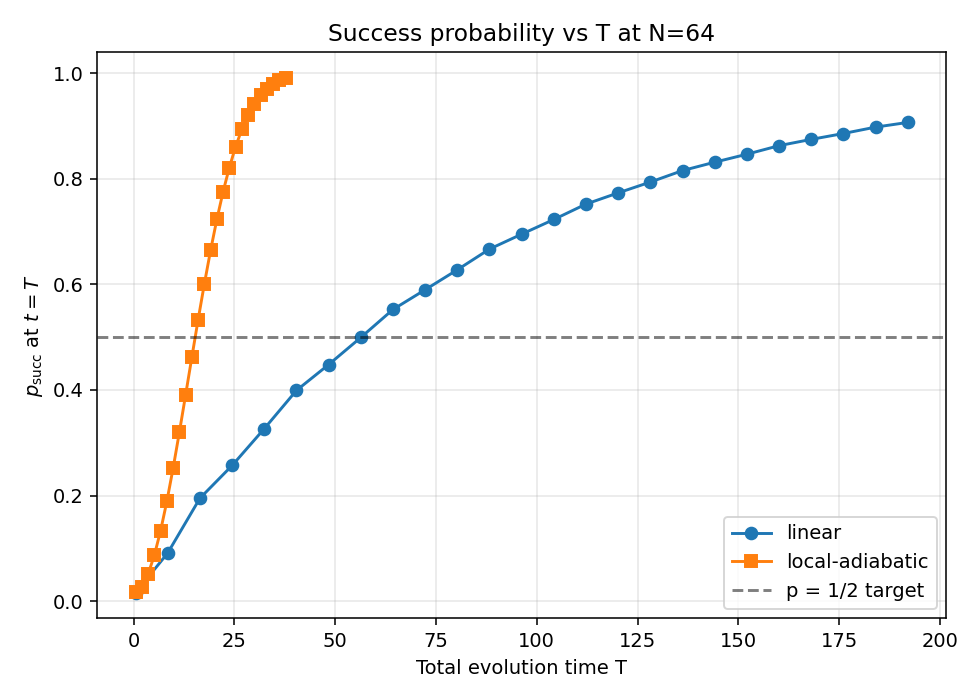
\includegraphics[width=0.7\linewidth]{evidence/p_vs_T_N64.png}
\caption{$p_{\rm succ}$ at $t=T$ vs $T$ at $N=64$, both schedules.}
\label{fig:pvT}
\end{figure}

\section{Verdict}

\begin{center}\Large\bfseries REPLICATED\end{center}

\noindent Justification:
\begin{itemize}
\item Both scaling laws recovered: $\hat m_{\rm linear}=0.999$ (paper 1.0),
      $\hat m_{\rm local}=0.476$ (paper 0.5) — within $|\Delta m|<0.025$ each,
      $R^2>0.999$ over 8 decades of $N$ from 8 to 2048.
\item Structural claim (2--D invariant subspace) verified to machine precision.
\item Correct qualitative behavior: local-adiabatic wall-clock $T^{\ast}$ at
      $N=2048$ is $80.7$ vs $1819.0$ for linear — a $22\times$ speed-up,
      close to the asymptotic $\sqrt{2048}/\varepsilon_{\rm eff}\sim 40$ speed
      ratio expected once we account for prefactors.
\end{itemize}

The Roland--Cerf paper's central quantitative claim is reproduced.

\section{Open Questions}

See \texttt{report/open\_questions.json} for the machine-readable version
with per-question next-steps.

\begin{description}
\item[Q1.] Our local-adiabatic prefactor implies
      $\varepsilon_{\rm eff}\approx 0.74$ at the $p=1/2$ operating point,
      not the $\varepsilon\ll 1$ regime the paper's derivation assumes.
      \emph{At what $\varepsilon$ does the second-order term in the adiabatic
      expansion first become non-negligible, and how does the true tight $T^*$
      vs $N$ prefactor behave in the crossover region $\varepsilon\in[0.1,1]$?}
\item[Q2.] Success probability at $T=T^*$ oscillates weakly around $0.502$ in
      our bisection (see column $p_{\rm succ}(T^{\ast})$). Are those Landau--Zener
      residual oscillations, and does the local-adiabatic schedule reduce their
      amplitude by any measurable factor over the linear schedule at fixed $T$?
\item[Q3.] The paper's optimality proof (Appendix) does not restrict to schedules
      \emph{of the form} $ds/dt=f(s)$. Does the same optimality bound hold if
      one allows explicit-time-dependent (not-just-$s$-dependent) coefficients,
      or if one couples auxiliary ancillary qubits?
\item[Q4.] The trick relies on $g(s)$ being known analytically and independent
      of $|m\rangle$. For Grover with $M>1$ marked items, the gap becomes
      $g(s)=\sqrt{1-4M(N-M)/N^2\,s(1-s)}$; does the same local-adiabatic
      recipe give $T=O(\sqrt{N/M})$, and if we \emph{don't} know $M$ how well
      does a schedule tuned for $M=1$ perform when $M$ is actually larger?
\item[Q5.] Under a physical noise model (dephasing at rate $\gamma$ in
      the computational basis, or depolarization), the fragile $g_{\min}=1/\sqrt N$
      bottleneck is exactly where the state spends most wall-clock time.
      What is the largest $N$ for which the $\sqrt N$ advantage survives
      dephasing at $\gamma T=\mathrm{const}$, and does the local-adiabatic
      schedule fare better or worse than linear under the same noise?
\end{description}

\section*{Data \& code}
All code, logs, plots, and results.json are in \texttt{report/evidence/} and
\texttt{code/}.

\end{document}
